% -*- TeX:de -*-
\NeedsTeXFormat{LaTeX2e}
\documentclass[12pt,a4paper]{article}
\usepackage[german]{babel} % german text
\usepackage[DIV12]{typearea} % size of printable area
\usepackage[T1]{fontenc} % font encoding
%\usepackage[latin1]{inputenc} % most likely on Windows
\usepackage[utf8]{inputenc} % probably on Linux
\usepackage{multicol}

% PLOTTING
\usepackage{pgfplots} 
\usepackage{pgfplotstable}
\usepackage{url}
\usepackage{graphicx} % to include images
\usepackage{tikz}
\usepackage{subfigure} % for creating subfigures
\usepackage{amsmath} % a bunch of symbols
\usepackage{amssymb} % even more symbols
\usepackage{booktabs} % pretty tables
\usepackage{makecell} % multi row table heading

% a floating environment for circuits
\usepackage{float}
\usepackage{caption}

%\newfloat{circuit}{tbph}{circuits}
%\floatname{circuit}{Schaltplan}

% a floating environment for diagrams
%\newfloat{diagram}{tbph}{diagrams}
%\floatname{diagram}{Diagramm}

\selectlanguage{german} % use german

\begin{document}

%%%%%%% DECKBLATT %%%%%%%
\thispagestyle{empty}
			\begin{center}
			\Large{Fakultät für Physik}\\
			\end{center}
\begin{verbatim}


\end{verbatim}
							%Eintrag des Wintersemesters
			\begin{center}
			\textbf{\LARGE WS 2013/14}
			\end{center}
\begin{verbatim}


\end{verbatim}
			\begin{center}
			\textbf{\LARGE{Physikalisches Praktikum\\ für das Bachelorstudium}}
			\end{center}
\begin{verbatim}




\end{verbatim}

			\begin{center}
			\textbf{\LARGE{PROTOKOLL}}
			\end{center}
			
\begin{verbatim}

\end{verbatim}

			\begin{flushleft}
			\textbf{\Large{Experiment (Nr., Titel):}}\\
							%Experiment Nr. und Titel statt den Punkten eintragen
			\LARGE{PW2 - Grundgrößen der Mechanik}	
			\end{flushleft}

\begin{verbatim}

\end{verbatim}	
							%Eintragen des Abgabedatums, oder des Erstelldatums des Protokolls
			\begin{flushleft}
			\textbf{\Large{Datum:}} \Large{23.1.2014}
			\end{flushleft}
			
\begin{verbatim}
\end{verbatim}
							%Namen der Protokollschreiber
		\begin{flushleft}
			\textbf{\Large{Namen:}} \Large{Patrick Braun, Johannes Kurz}
			\end{flushleft}

\begin{verbatim}


\end{verbatim}
							%Kurstag und Gruppennummer, zb. Fr/5
			\begin{flushleft}
			\textbf{\Large{Kurstag/Gruppe:}} \Large{DO/2}
			\end{flushleft}

\begin{verbatim}

\end{verbatim}
							%Name des Betreuers, das Praktikum betreute.
			\begin{flushleft}
			\LARGE{\textbf{Betreuer:}}	\Large{Franz Sachslehner}	
			\end{flushleft}

%%%%%%% DECKBLATT ENDE %%%%%%%
\pagebreak
\setlength{\columnsep}{20pt}
\begin{multicols}{2}

%%%%%%%%%%%%%%%%%%%%%%%%%%%%%%%%%%%%%%%%%%%%%%%%

%\begin{figure}[H]
%	\centering
%	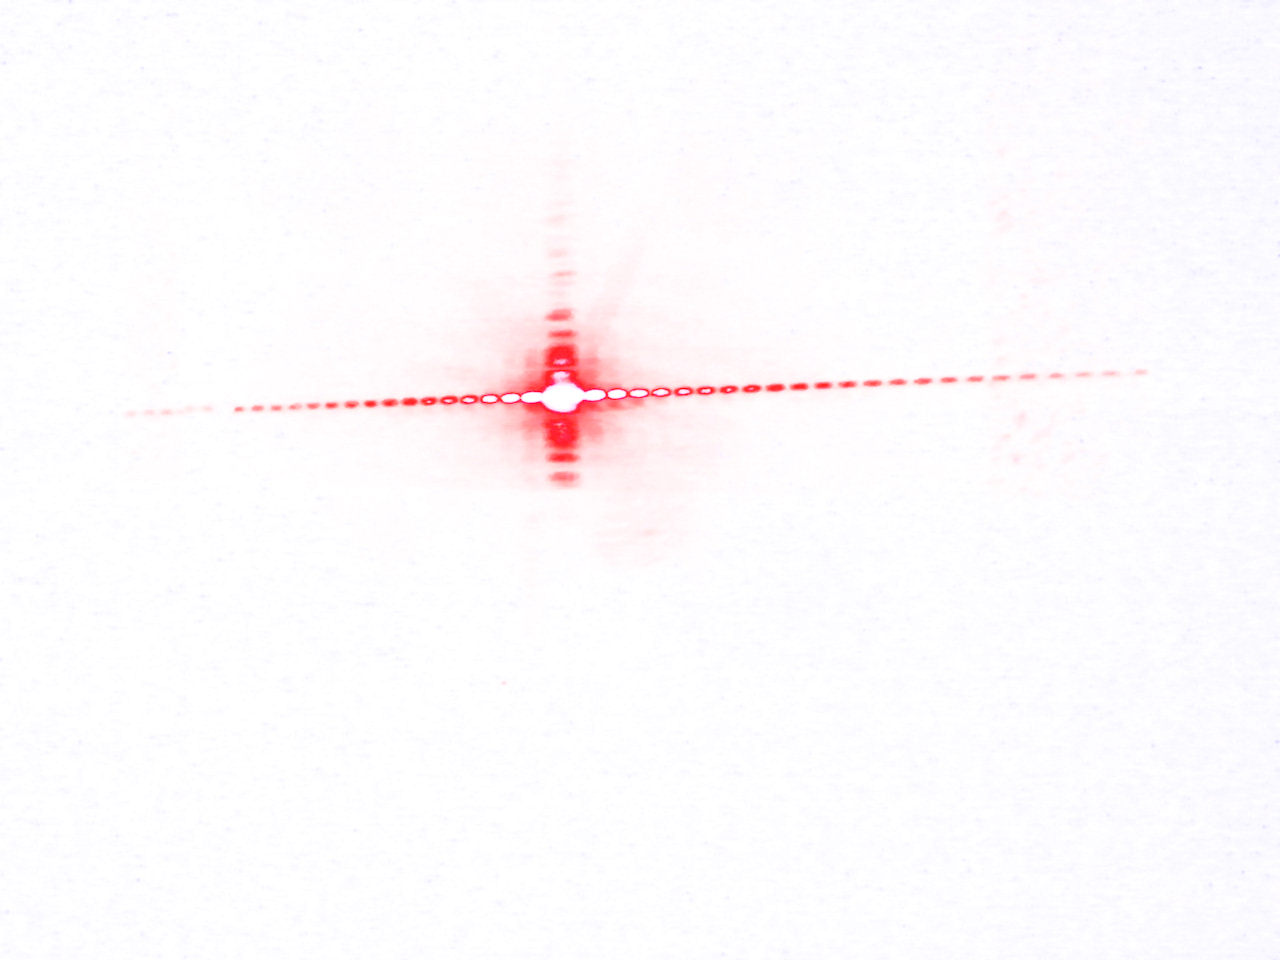
\includegraphics[scale=0.35]{./figure/beugung.png}
%	\caption{Beugungsmuster Einzelspalt (echtes Foto; schwarz durch weiß ersetzt)}
%	\label{fig:beugungsmuster}
%\end{figure}


%\begin{figure}[H]
%	\centering
%	\pgfplotstabletypeset[
%			columns={abstand, n},
%			col sep=&,
%			columns/abstand/.style={precision=2, zerofill, column name=\makecell{$Abstand$\\$(\pm 0.05)[mm]$} }, 
%			columns/n/.style={column name=\makecell{$n$\\$(Ordnung)$}, precision=0},
%			every head row/.style={before row=\hline,after row=\hline\hline},
%			every last row/.style={after row=\hline},
%			every first column/.style={column type/.add={|}{} },
%			every last column/.style={column type/.add={}{|} }
%			]{
%			abstand & n
%			12.9 & 1
%			24.45 & 2
%			37.40 & 3
%			49.35& 4
%			62.45 & 5
%			74.45 & 6
%			87.45 & 7
%			100.25 & 8
%			
%			}
%	\caption{Messwerte Einzelspalt}
%	\label{tab:werte_einzelspalt}
%\end{figure}
%

%%%%%%%%%%%%%%%%%%%%%%%%%%%%%%%%%%%%%%%%
\section{Dichte von Flüssigkeiten}

\subsection{Theorie}

Im ersten Teil von PW2 soll die Dichte einer Flüssigkeit (Kupfersulfat-Lösung) auf 3 verschiedene Arten bestimmt werden, und diese verglichen werden.\\
Die Dichte $\rho$ ist die Masse pro Volumseinheit eines Körpers oder eines Fluids. Im Falle einer homogenen Masseverteilung, wie in diesem Experiment, gilt
$$\rho = \frac{m}{V}$$

Bei gleichem Volumen verhalten sich also die Massen 2er verschiedener Stoffe zueinander genauso, wie deren Dichten.\\
Sind die untersuchten Stoffe keine Festkörper, wirken auf einen in das jeweilige Fluid eingetauchten Senkkörper eine Auftriebskraft. Die Auftriebskräfte verhalten sich ebenso zueinander, wie die Dichten.\\
Hier wird jedoch durch Messung der Masse der verdrängten Flüssigkeit, bei bekanntem Volumen des Senkkörpers, die Dichtemessung durchgeführt.

%Diese beiden Verhältnisse werden benützt um, einmal im Vergleich mit destilliertem Wasser, einmal mit Luft, die Dichte der Testflüssigkeit zu bestimmen.

%$$\rho = \frac{M}{V} = \frac{[kg]}{[m^3]}$$


\subsection{Aufbau und Methoden}
\textbf{Messung mit dem Pyknometer:}\\
Das Pyknometer ist ein Gefäß, um sehr genau bestimmte Volumina eines Fluides einzufüllen. Würden in einem beliebigen Gefäß mit einer größeren Öffnung, die verschiedenen Oberflächenspannungen es zum Ratespiel machen, gleiche Volumina verschiedener Flüssigkeiten einzufüllen, sorgt hier ein genau eingepasster Stöpsel mit Kapillarbohrung dafür, diesen Einfluss praktisch zu eliminieren.\\
Zuerst wird die Masse $m_0$ des leere Gefäßes gemessen, danach das zu messende Fluid eingefüllt. Ist der Verschluss aufgesetzt, muss für eine genaue Messung sämtliche überschüssige Flüssigkeit vom Gefäß und von der Kapillaröffnung beseitigt werden.\\
So werden die Massen von, in guter Näherung gleichen, Volumina von destilliertem Wasser ($m_1$) und der Kupfersulfatlösung ($m_2$) bestimmt.\\
Die Dichte ergibt sich durch:
$$\rho_{Probe}=\frac{m_2-m_0}{m_1-m_0}\cdot \rho_{dest.}$$
Die Dichte des destillierten Wassers $\rho_{dest}$ wird, nach Messung der Raumtemperatur, aus einer Tabelle entnommen.\\
\\
\textbf{Messung mittels Waage:}\\
Auf einer Waage wird ein Galgen montiert, an dem ein Senkkörper angebracht wird ($Volumen=10cm^3$). Dabei ist darauf zu achten, die Waage waagrecht einzurichten, danach wird sie, mit dem Senkkörper frei in der Raumluft hängend, tariert.\\
Anschließend wird ein Gefäß mit der Probeflüssigkeit so unter den Senkkörper gebracht, dass dieser zur Gänze in das Fluid eintaucht. Der Aufbau ist dabei so zu konstruieren, dass die Waage ausschließlich die Gewichtskraft misst, die auf den Senkkörper wirkt, und nicht die des Gefäßes.\\
Die Auftriebskraft auf den Senkkörper wird nun als negatives Gewicht angezeigt. Eigentlich misst die Waage jedoch die Masse der verdrängten Flüssigkeit. Bei bekanntem Volumen des Senkkörpers ergibt sich dadurch die Dichte.\\
\\
\textbf{Digital-Densiometer:}\\
Zuletzt soll die Dichte der Flüssigkeit mit einem Gerät, speziell zur Dichtemessung, bestimmt werden.\\
Dieses gibt direkt eine gemessene Dichte aus.\\
Es ist nur darauf zu achten, die Probenkammer mit der zu messenden Flüssigkeit auszuspülen, um Verunreinigungen zu minimieren.

\subsection{Resultate}

\textbf{Pyknometer:}\\
Leeres Gefäß: $m_0 = (31.4 \pm 0.1)g$\\
mit dest. Wasser: $m_1 = (82.7 \pm 0.1)g$\\
Probeflüssigkeit: $m_2 = (84.6 \pm 0.1)g$\\
\\
Temperatur $T_{dest} = 22.9^\circ \pm 0.1^\circ$\\
$\rho_{dest} = 997.560 \pm 0.025) kg/m^3$
$$\rho_{Probe} = (1034.5 \pm 2.1) kg/m^3$$\\



\noindent \textbf{Auftrieb:}\\

\noindent Volumen des Probekörpers: 10 $cm^3$\\
Verdrängte Flüssigkeit:\\
%dest. Wasser: $m_{Wasser} = (9.973 \pm 0.001)g$\\
%$m_{Probe} = (10.347 \pm 0.001)g$\\
$$\rho_{Probe} = (1034.7 \pm 0.1)g$$\\
Nach der Korrektur des Auftriebs durch die Luft:\\
$$\rho_{korrig.} = (1033.5 \pm 0.1)g$$\\



\textbf{Densiometer}
%4 Messungen:
%$$\rho_{1.1}:   (1.0347 \pm 0.001) \frac{g}{cm^3}$$
%$$\rho_{1.2}:   (1.0366 \pm 0.001) \frac{g}{cm^3}$$
%Gereinigt:
%$$\rho_{2.1}:   (1.0366 \pm 0.001) \frac{g}{cm^3}$$
$$\rho_{2.2}:   (1.0364 \pm 0.001) \frac{g}{cm^3}$$
\subsection{Diskussion}

%Densiometer.. 4 Messungen.. erste nicht so toll

%%%%%%%%%%%%%%%%%%%%%%%%%%%%%%%%%%%%%%%%
\section{Gleichmäßig beschleunigte Bewegung, eindimensional}

\subsection{Theorie}

g \ldots Gravitationsbeschleunigung Erde\\
m \ldots kleine Masse am Faden\\
M \ldots große Masse am Tisch\\
$\mu$ \ldots Reibungskoeffizient von M\\
a \ldots Beschleunigung beider Massen\\

$$F_g = m * g = [N]$$
$$F_{Reibung} = M*g*\mu$$
$$F_{mM} = (m+M)*a$$
$$F_{g} = F_{mM} + F_{Reibung}$$
$$m * g = M*g*\mu + (m+M)*a$$

\subsection{Aufbau und Methoden}

\subsection{Resultate}
Polynomieller Fit x-ter Ordnung mit der Formel:
$$x(t) = A_0 + B_1*t^1 + B_2 * t^2$$
$$v(t) = B_1 + B_2 * 2 * t$$
$$a(t) = B_2 * 2 = const$$
\end{multicols}
\begin{figure}[H]
	\centering
	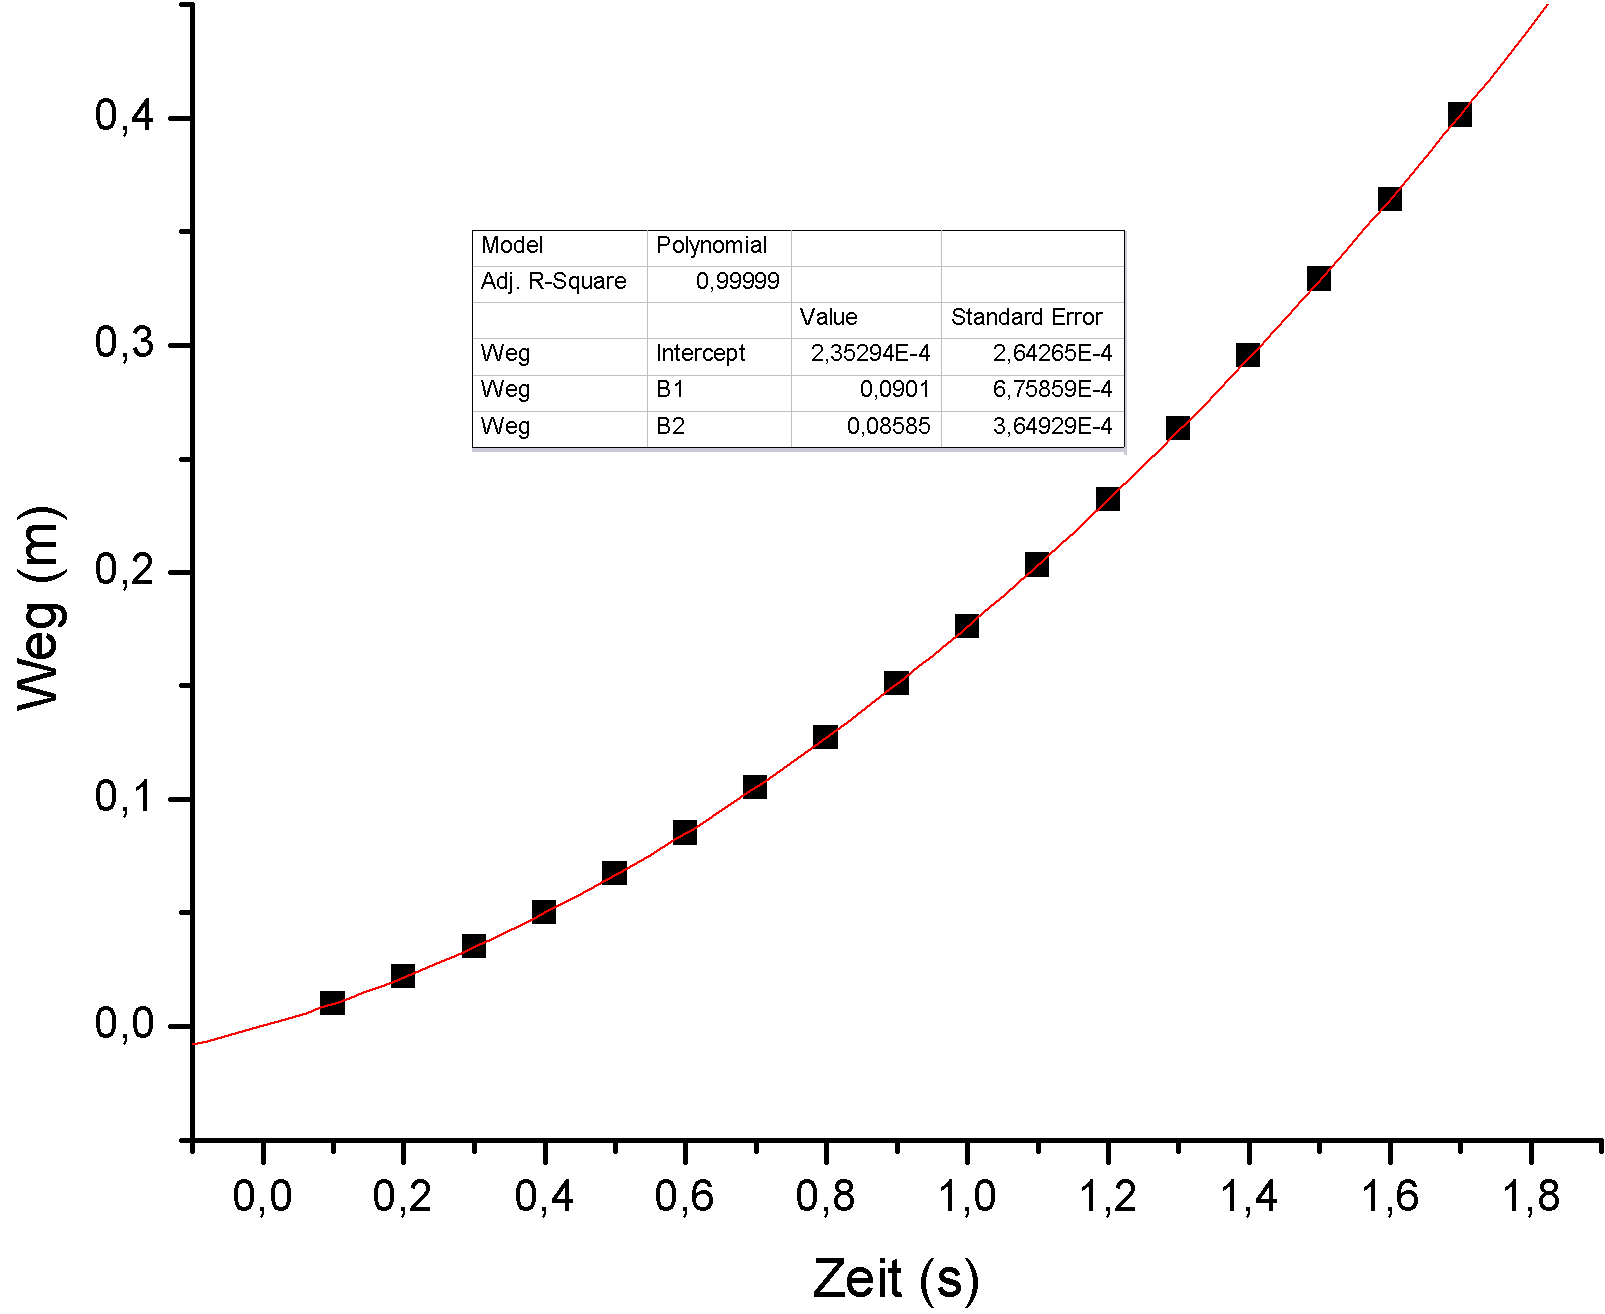
\includegraphics[scale=0.4]{./figure/x_t_diagram.png}
	\caption{x(t)-Diagram}
	\label{fig:lin_bewegung}
\end{figure}
\begin{figure}[H]
	\centering
	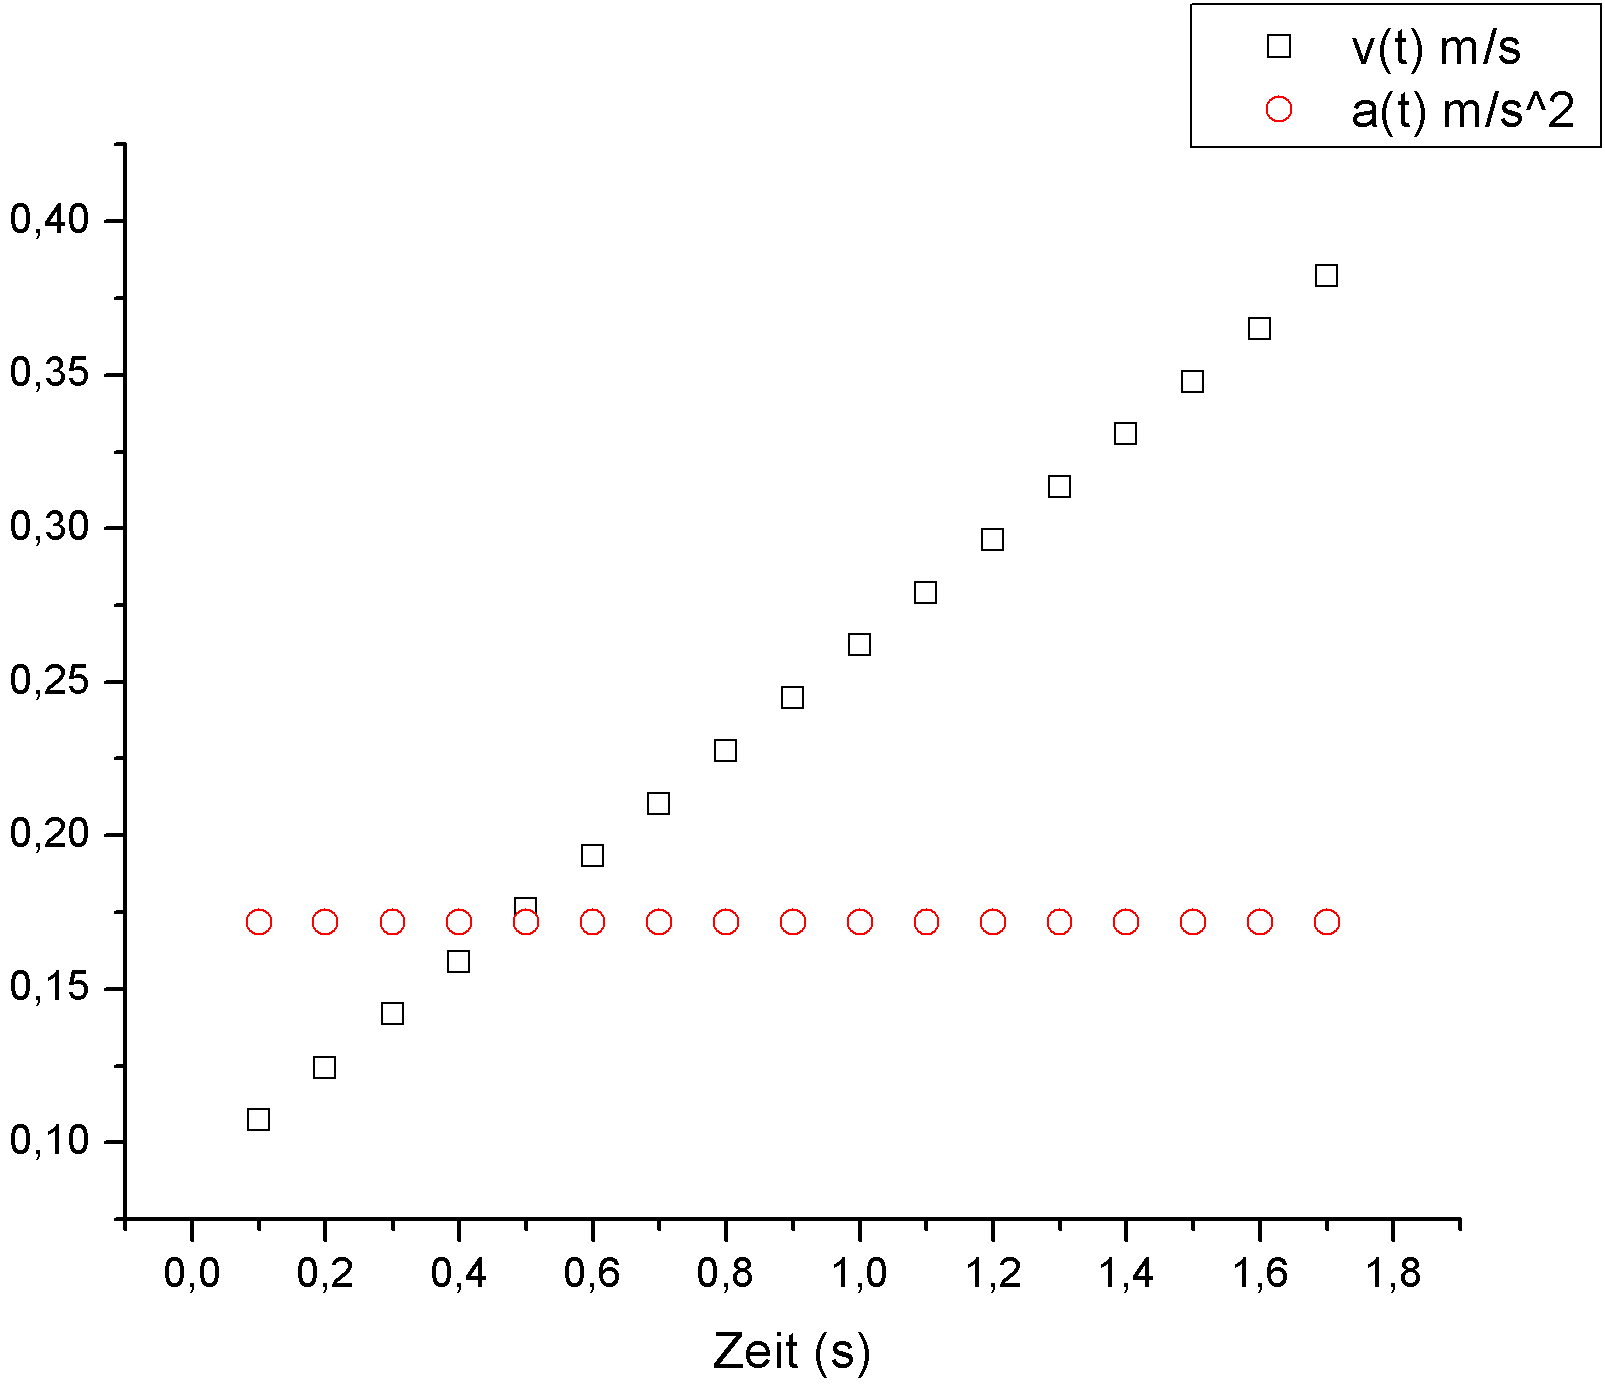
\includegraphics[scale=0.4]{./figure/v_a_t_diagram.png}
	\caption{v(t)-Diagram und a(t)-Diagram}
	\label{fig:lin_bewegung_v_a}
\end{figure}
\begin{multicols}{2}

\subsection{Diskussion}

\end{multicols}

\begin{figure}[H]
	\centering
	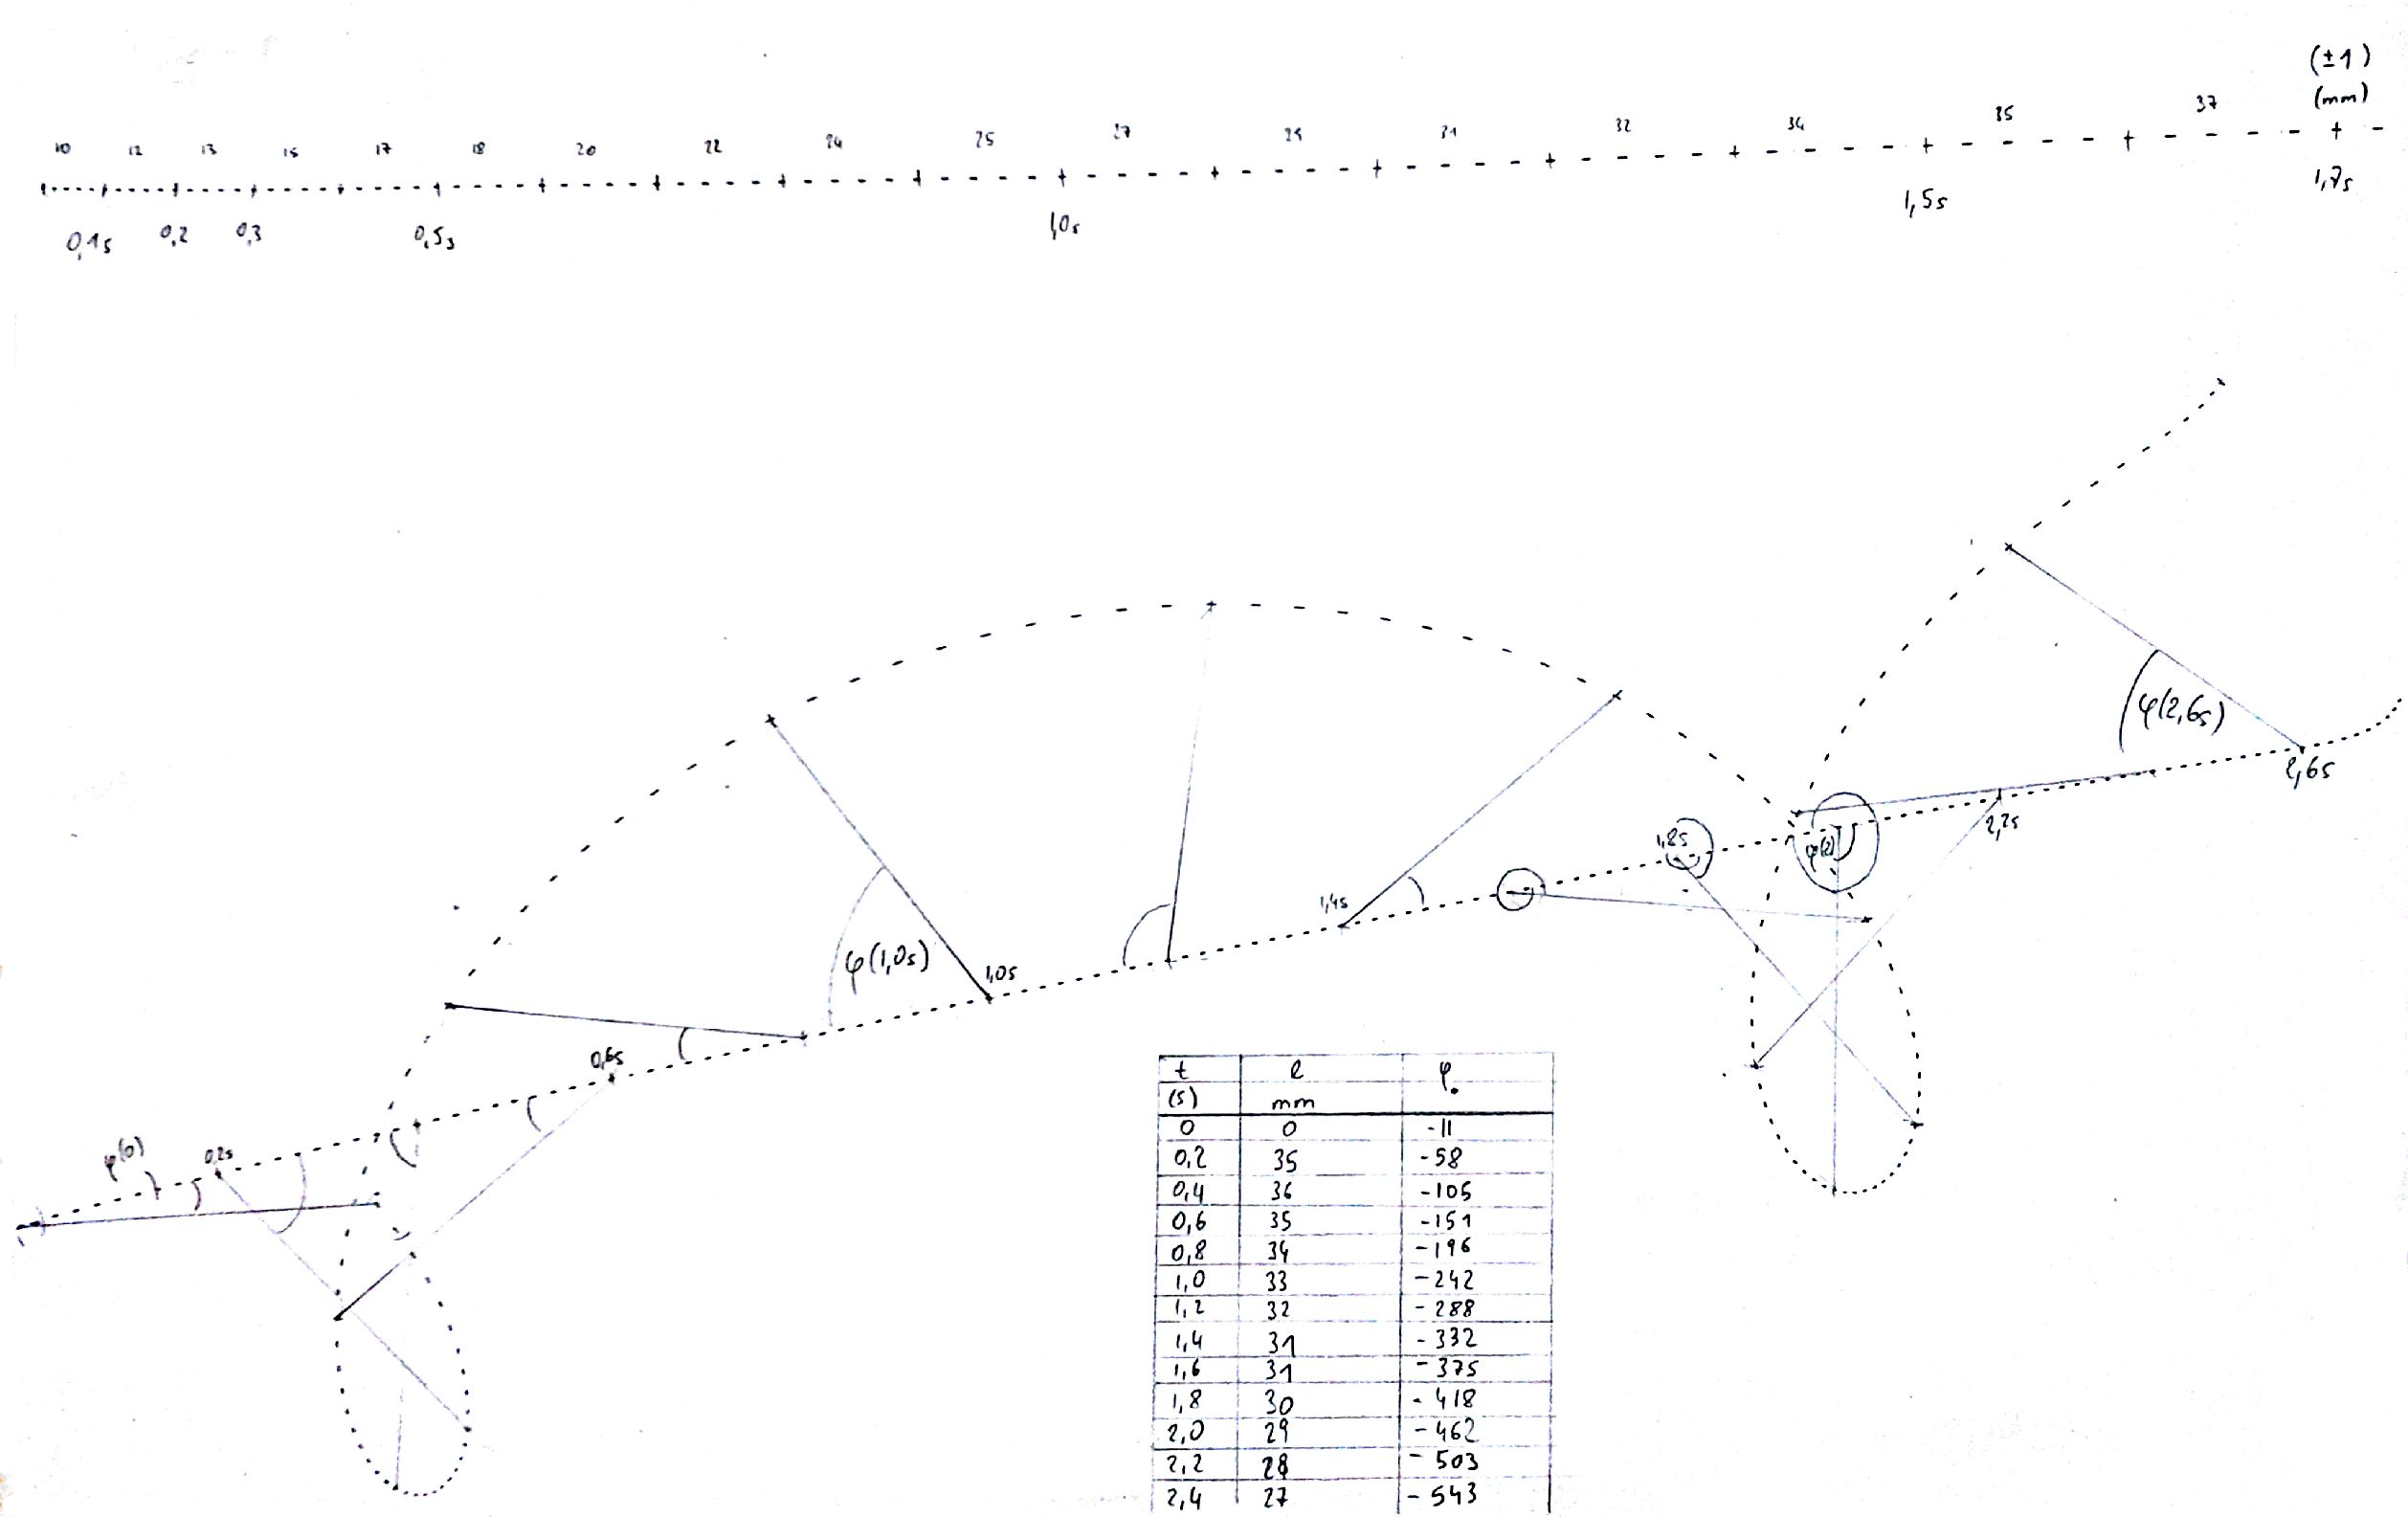
\includegraphics[scale=0.25, angle=-90]{./figure/bewegungen.jpg}
	\caption{Eindimensionale Beschleunigung und kräftefreie Bewegung}
	\label{fig:bewegungen}
\end{figure}

\begin{multicols}{2}
%%%%%%%%%%%%%%%%%%%%%%%%%%%%%%%%%%%%%%%%
\section{Kräftefreie Bewegung}

\subsection{Theorie}

\subsection{Aufbau und Methoden}

\subsection{Resultate}

\subsection{Diskussion}


%%%%%%%%%%%%%%%%%%%%%%%%%%%%%%%%%%%%%%%%
\section{Elastischer Stoß}

\subsection{Theorie}

\subsection{Aufbau und Methoden}

\subsection{Resultate}

\subsection{Diskussion}



%%%%%%%%%%%%%%%%%%%%%%%%%%%%%%%%%%%%%%%%
\section{Inelastischer Stoß}

\subsection{Theorie}

\subsection{Aufbau und Methoden}

\subsection{Resultate}

\subsection{Diskussion}


\section{Quellen}
$[1]$ Anleitung, \url{http://www.univie.ac.at/anfpra/neu1/pw/pw2/PW2.pdf}\\
\end{multicols}

\end{document}